\documentclass[12pt]{article}
\usepackage[utf8]{inputenc}
\usepackage[spanish]{babel}
\usepackage{graphicx}
\usepackage{hyperref}
\usepackage{todonotes}
\hypersetup{
    colorlinks=true,
    linkcolor=cyan,
    filecolor=magenta,      
    urlcolor=blue,
    }

\title{Famtime Food\\\emph{Rien de mieux que la famille.}}
\author{Victor Chavarria, Samuel Gutierrez, Jonathan Zavala, Grecia Morales}
\date{Septiembre - Diciembre, 2023}

\begin{document}

\maketitle

\newpage
\section {Acerca del proyecto}
\p Este es una idea de proyecto donde se busca optimizar el tiempo de respuesta del restaurante o cafeter�a, donde los clientes al llegar ya tengan su orden lista, y solo con ligar el turno con el pedido del cliente a una mesa dentro del recinto, se evita que tengan que gastar tiempo en ver el menu, ponerse de acuerdo, esperar al mesero, etc.

\newpage
\tableofcontents
\newpage

\section {REQUERIMIENTOS FUNCIONALES}

\subsection {Cliente}
\begin{itemize}
  \item Seleccionar categorias de comida.
	\item Seleccionar la comida.
	\item Revisar el pedido.
	\item Selecciona complementos al pedido.
	\item Confirmar pedido.
	\item Editar pedido.
	\item Editar cantidades de comida.
	\item Obtener turno.
	\item Guardar turno en dispositivo.
	\item Recibir notificaciones del estado del pedido.
	\item Regresar al menu.
\end{itemize}

\subsection {Recepcionista}
\begin{itemize}
	\item Recibe el pedido del cliente.
	\item Liga el turno/pedido del cliente con la mesa disponible.
\end{itemize}

\subsection {Cocina}
\begin{itemize}
	\item Recibe el pedido.
	\item Selecciona el  pedido.
	\item Marcar pedido como completado.
	\item Notificar que el pedido ya est� listo.
\end{itemize}

\section {REQUERIMIENTO NO FUNCIONAL}
\begin{itemize}
  \item Desarrollo en VSC.
	\item Framework Bootstrap.
	\item JS, HTML, CSS.
	\item Framework Laravel php.
	\item Uso de internet para la app.
	\item Acceso al carrete (Guardado del pedido).
	\item Acceso a las notificaciones (estado de los pedidos).
\end{itemize}

\newpage
\section {CASOS DE USO:}
\subsection {Diagrama}
\begin{figure}[htbp]
	\centering
		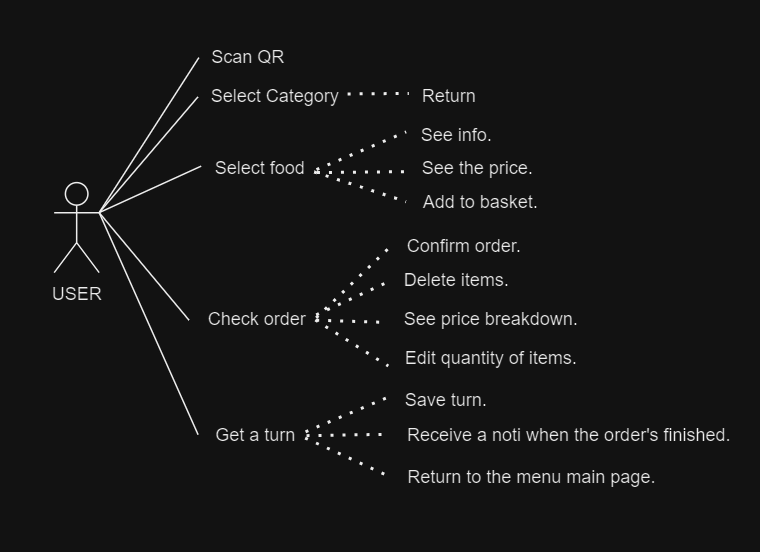
\includegraphics[width=1.00\textwidth]{C:/xampp/htdocs/Cafeteria-Menu/docImg/Img/Diagrams/DiagramaCasos/Diagrama-casos-user.png}
	\caption{Diagrama de casos usuario}
	\label{fig:Diagrama-casos-user}
\end{figure}


\begin{figure}[htbp]
	\centering
		
\includegraphics[width=1.00\textwidth]{C:/xampp/htdocs/Cafeteria-Menu/docImg/Img/Diagrams/DiagramaCasos/Diagrama-casos-receptionist.png}
	\caption{Diagrama de casos recepcionista}
	\label{fig:Diagrama-casos-receptionist}
\end{figure}

\begin{figure}[htbp]
	\centering
		
\includegraphics[width=1.00\textwidth]{C:/xampp/htdocs/Cafeteria-Menu/docImg/Img/Diagrams/DiagramaCasos/Diagrama-casos-kitchen.png}
	\caption{Diagrama de casos cocina}
	\label{fig:Diagrama-casos-kitchen}
\end{figure}


\newpage
\subsection {Flujo ideal}
\begin{itemize}
  \item Escanear QR.
	\item LogIn / SignUp.
  \item Seleccionar una categor�a.
  \item Seleccionar un alimento.
  \item Agregar a la canasta.
	\item Revisar su pedido.
	\item Obtener tu turno.
\end{itemize}

\subsection {Flujo alterno}
\begin{itemize}
	\item Escanear QR.
	\item LogIn / SignUp.
  \item Seleccionar una categor�a.
		\subitem Revisar tu canasta.
  \item Seleccionar un alimento.
		\subitem Revisar la informaci�n del alimento.
		\subitem Agregar el alimento a la canasta.
		\subitem Revisar la canasta.
		\subitem Regresar a la selecci�n de categor�as.
  \item Revisar pedido.
		\subitem Regresar a la selecci�n de categor�as.
		\subitem Confirmar pedido.
		\subitem Editar cantidades de item.
		\subitem Eliminar items.
	\item Obtener tu turno.
		\subitem Guardar turno en carrete.
		\subitem Regresar al menu.
\end{itemize}

\newpage
\section {DIAGRAMAS}
\subsection {Diagrama de componentes}
\begin{figure}[htbp]
	\centering
		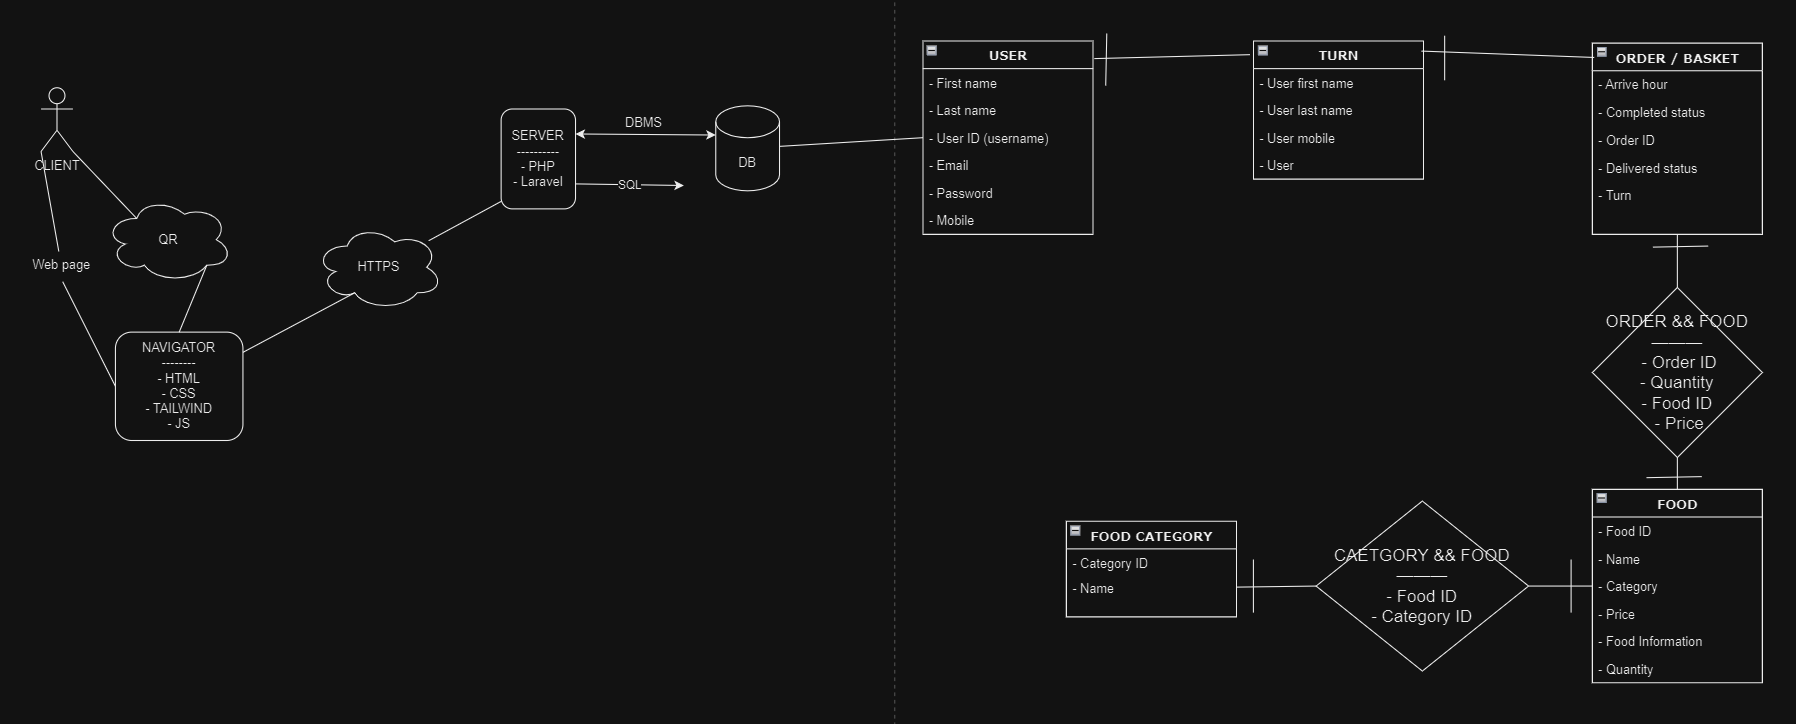
\includegraphics[width=1.00\textwidth]{C:/xampp/htdocs/Cafeteria-Menu/docImg/Img/Diagrams/DiagramaComponentes/Diagrama-componentes-general.png}
	\caption{Diagrama-componentes-general}
	\label{fig:Diagrama-componentes-general}
\end{figure}


\subsection {Diagrama de clases}
\begin{figure}[htbp]
	\centering
		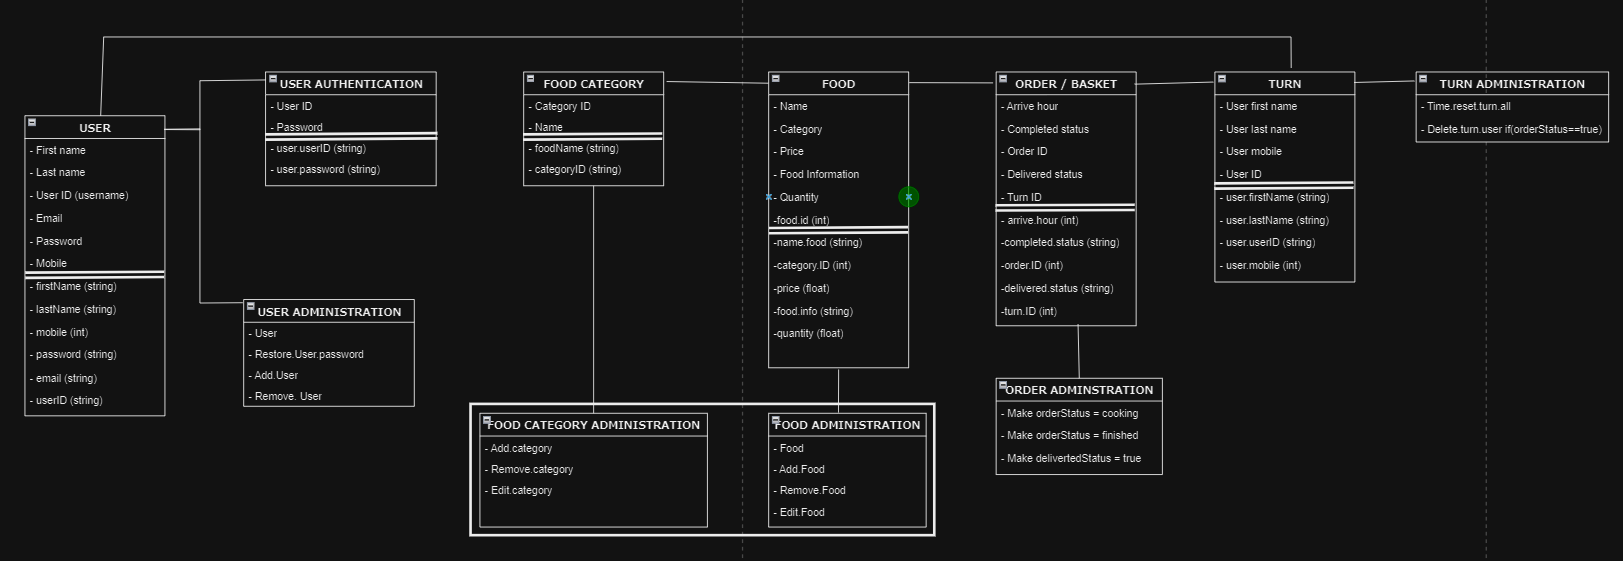
\includegraphics[width=1.00\textwidth]{C:/xampp/htdocs/Cafeteria-Menu/docImg/Img/Diagrams/DiagramaClases/Diagrama-clases-general.png}
	\caption{Diagrama de clases}
	\label{fig:Diagrama-clases-general}
\end{figure}


\newpage

\subsection {Diagrama de secuencia}
\begin{figure}[htbp]
	\centering
		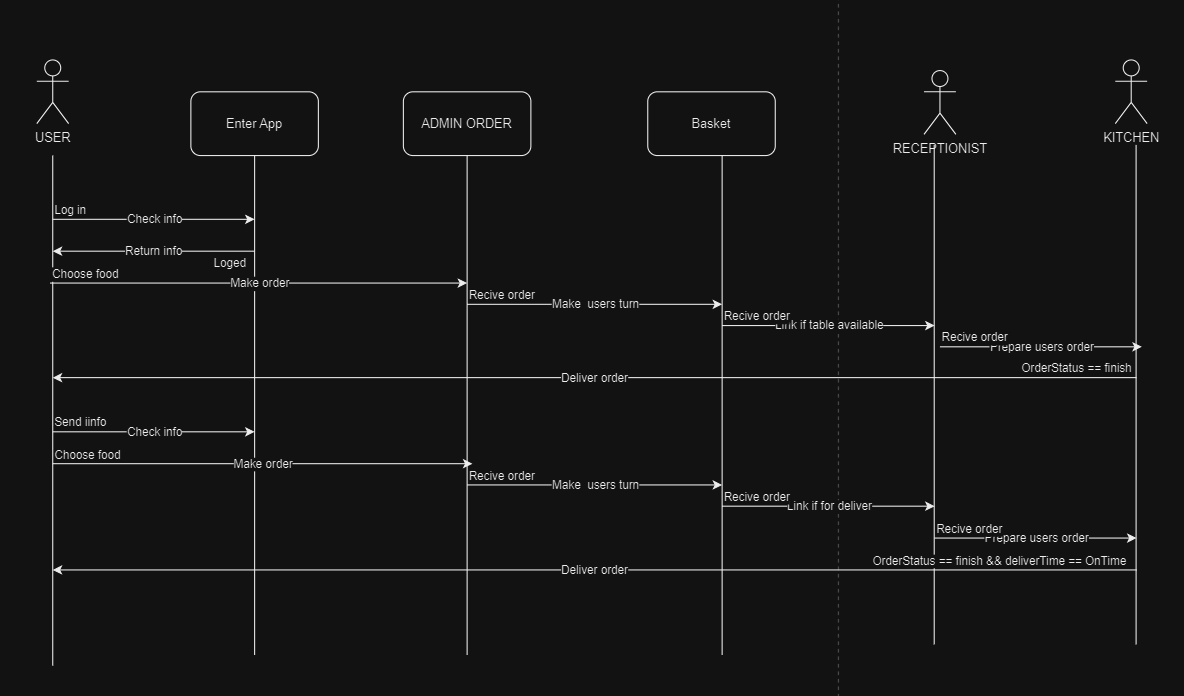
\includegraphics[width=1.00\textwidth]{C:/xampp/htdocs/Cafeteria-Menu/docImg/Img/Diagrams/DiagramaSecuencia/Diagrama-secuencia-general.png}
	\caption{Diagrama de secuencia general}
	\label{fig:Diagrama-secuencia-agregar-comida}
\end{figure}

\begin{figure}[htbp]
	\centering
		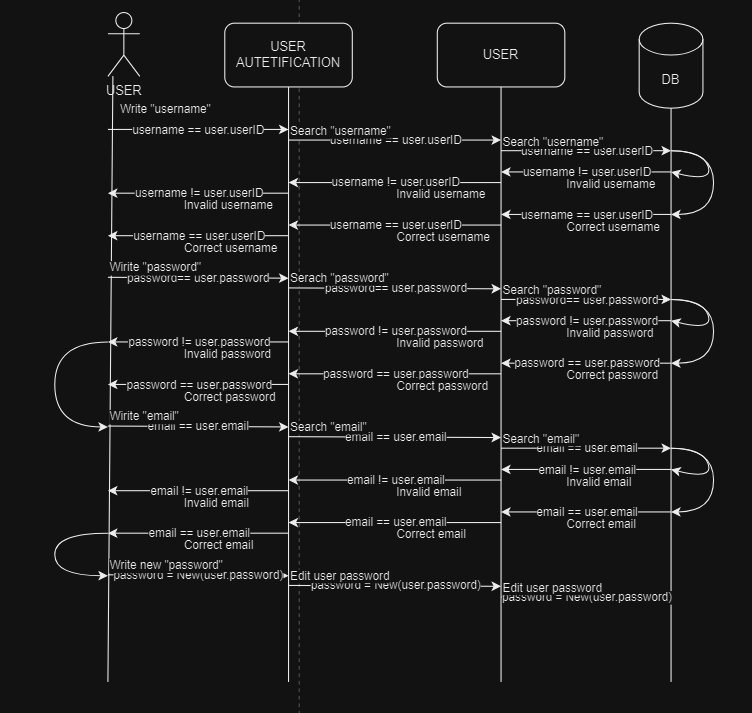
\includegraphics[width=1.00\textwidth]{C:/xampp/htdocs/Cafeteria-Menu/docImg/Img/Diagrams/DiagramaSecuencia/Diagrama-secuencia-LogIn.png}
	\caption{Diagrama secuencia LogIn}
	\label{fig:Diagrama-secuencia-LogIn}
\end{figure}

\begin{figure}[htbp]
	\centering
		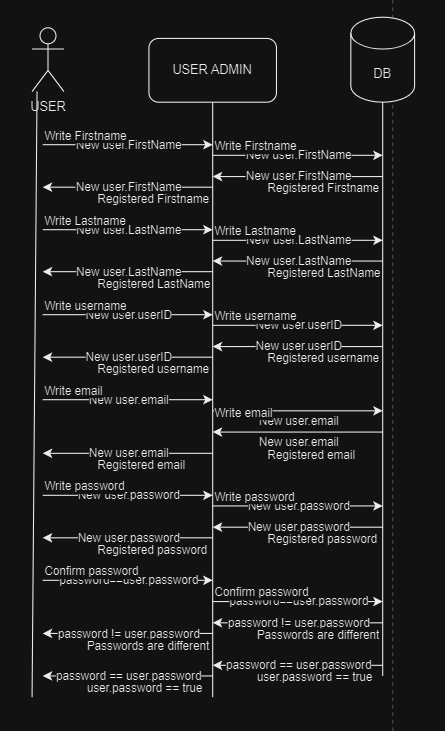
\includegraphics[width=0.80\textwidth]{C:/xampp/htdocs/Cafeteria-Menu/docImg/Img/Diagrams/DiagramaSecuencia/Diagrama-secuencia-SignUp.png}
	\caption{Diagrama secuencia SignUp}
	\label{fig:Diagrama-secuencia-SignUp}
\end{figure}

\begin{figure}[htbp]
	\centering
		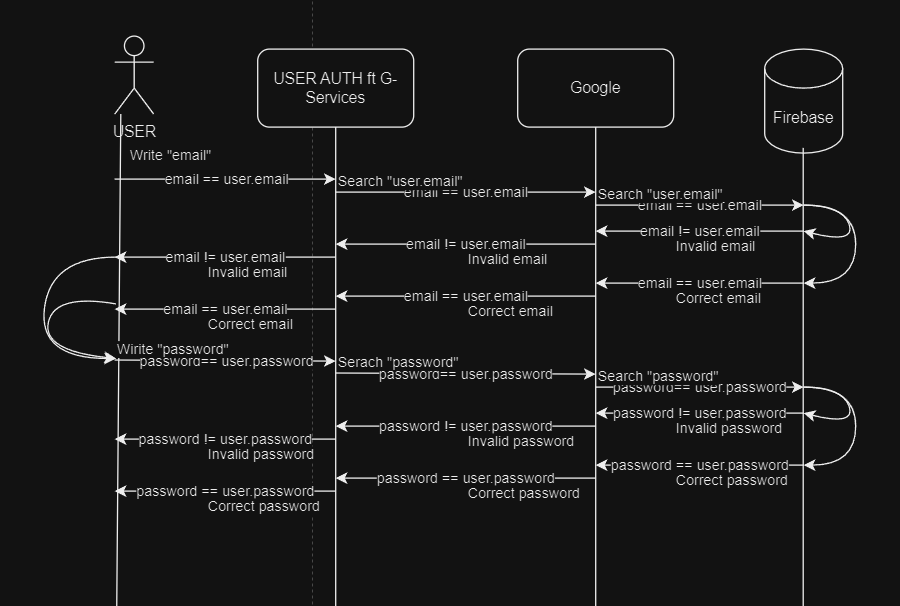
\includegraphics[width=1.00\textwidth]{C:/xampp/htdocs/Cafeteria-Menu/docImg/Img/Diagrams/DiagramasFlujo/DiagramaFlujo-SignUp-Google.png}
	\caption{Diagrama secuencia SignUp y LogIn con Google Services}
	\label{fig:DiagramaFlujo-SignUp-Google}
\end{figure}

\begin{figure}[htbp]
	\centering
		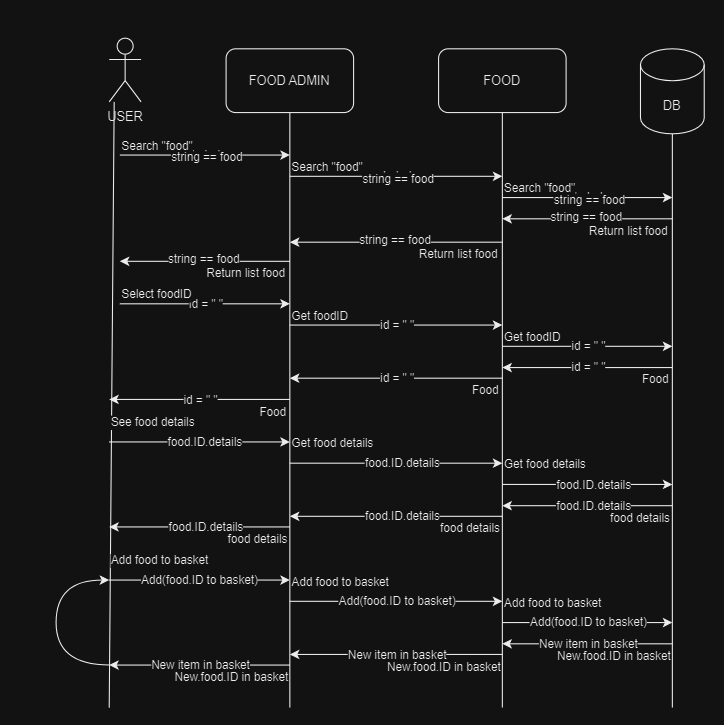
\includegraphics[width=1.00\textwidth]{C:/xampp/htdocs/Cafeteria-Menu/docImg/Img/Diagrams/DiagramaSecuencia/Diagrama-secuencia-agregar-comida.png}
	\caption{Diagrama secuencia pedir comida}
	\label{fig:Diagrama-secuencia-agregar-comida}
\end{figure}

\begin{figure}[htbp]
	\centering
		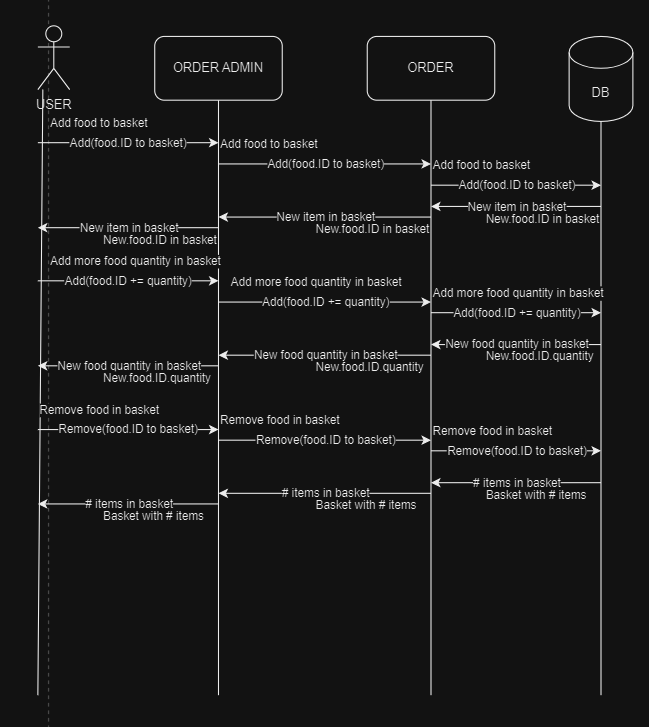
\includegraphics[width=1.00\textwidth]{C:/xampp/htdocs/Cafeteria-Menu/docImg/Img/Diagrams/DiagramaSecuencia/Diagrama-secuencia-orders.png}
	\caption{Diagrama secuencia ordenes}
	\label{fig:Diagrama-secuencia-orders}
\end{figure}


\newpage

\subsection {Diagrama de flujo}
\begin{figure}[htbp]
	\centering
		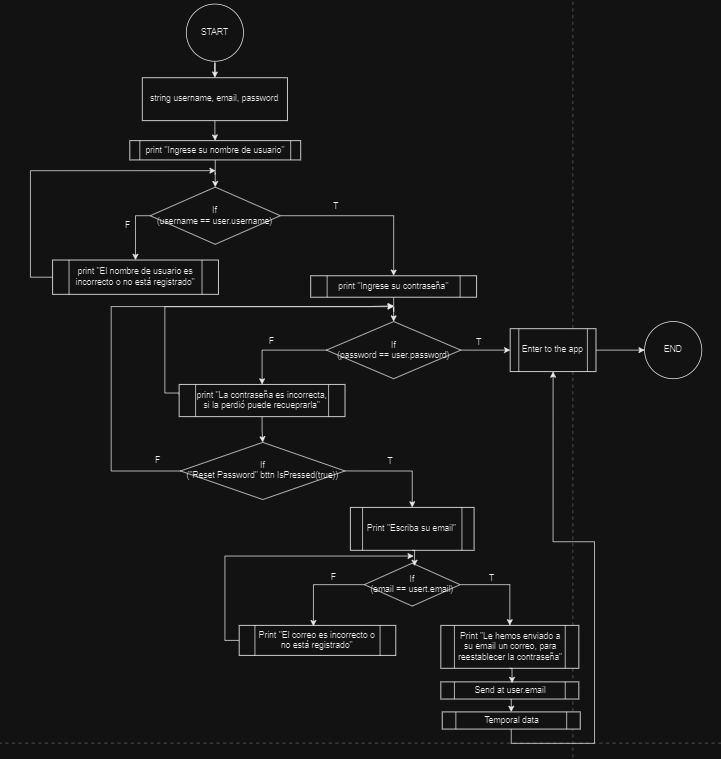
\includegraphics[width=0.90\textwidth]{C:/xampp/htdocs/Cafeteria-Menu/docImg/Img/Diagrams/DiagramasFlujo/DiagramaFlujo-LogIn.png}
	\caption{Diagrama de flujo LogIn}
	\label{fig:DiagramaFlujo-LogIn}
\end{figure}

\begin{figure}[htbp]
	\centering
		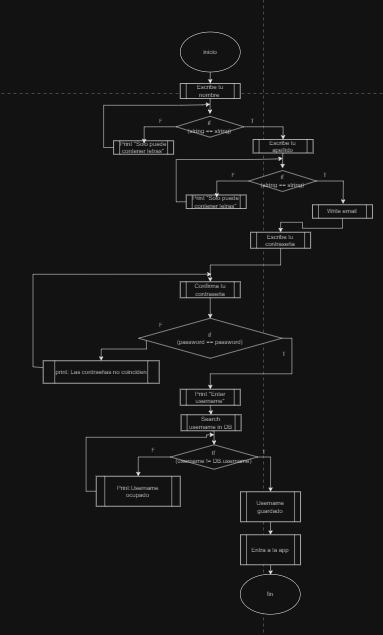
\includegraphics[width=0.80\textwidth]{C:/xampp/htdocs/Cafeteria-Menu/docImg/Img/Diagrams/DiagramasFlujo/DiagramaFlujo-SignUp.png}
	\caption{Diagrama de flujo SignUp}
	\label{fig:DiagramaFlujo-SignUp}
\end{figure}

\begin{figure}[htbp]
	\centering
		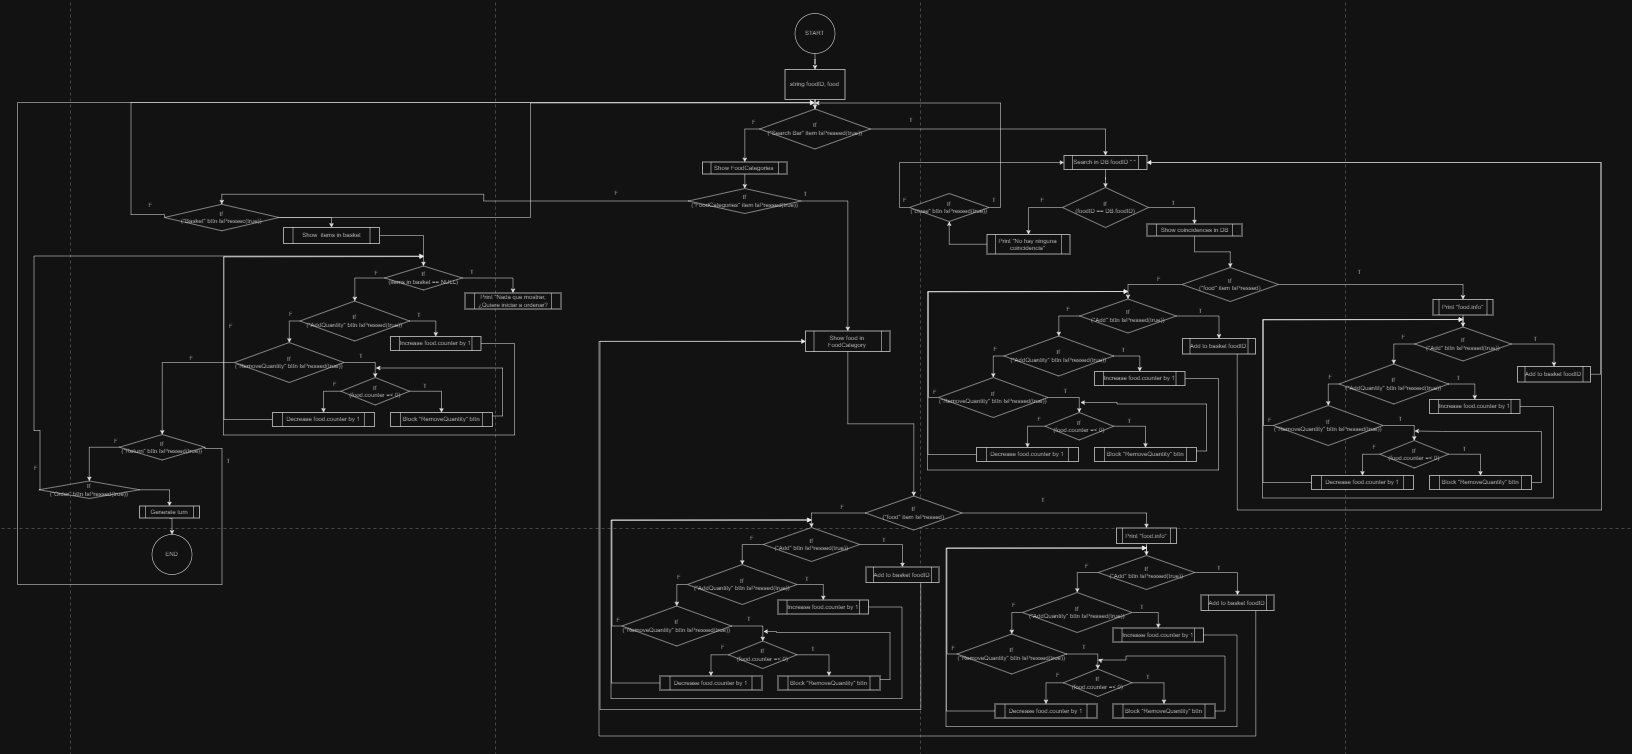
\includegraphics[width=1.00\textwidth]{C:/xampp/htdocs/Cafeteria-Menu/docImg/Img/Diagrams/DiagramasFlujo/DiagramaFlujo-UI.png}
	\caption{Diagrama de flujo UI}
	\label{fig:DiagramaFlujo-UI}
\end{figure}

\begin{figure}[htbp]
	\centering
		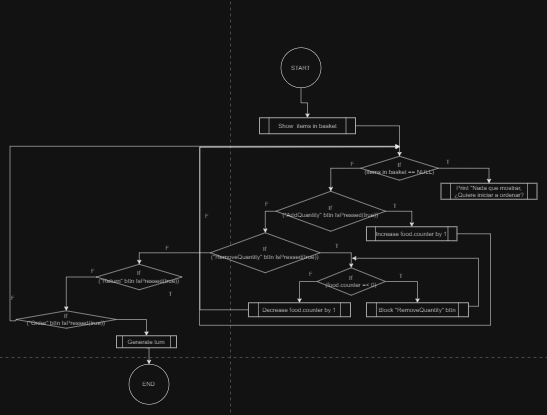
\includegraphics[width=1.00\textwidth]{C:/xampp/htdocs/Cafeteria-Menu/docImg/Img/Diagrams/DiagramasFlujo/DiagramFlujo-Basket.png}
	\caption{Diagrama de flujo Basket}
	\label{fig:DiagramFlujo-Basket}
\end{figure}

\newpage

\subsection {Diagrama de estados}
\begin{figure}[htbp]
	\centering
		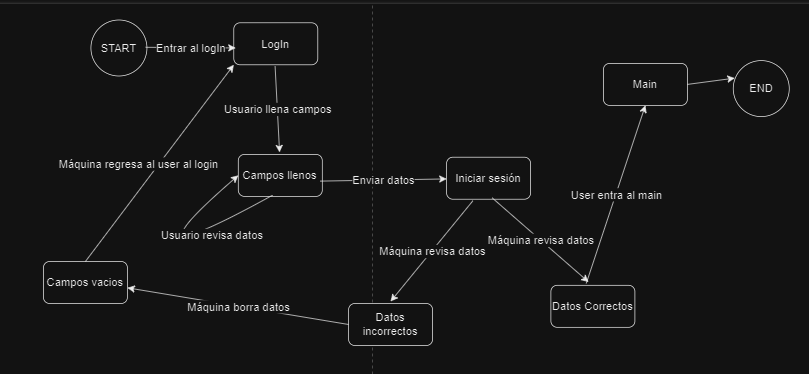
\includegraphics[width=1.00\textwidth]{C:/xampp/htdocs/Cafeteria-Menu/docImg/Img/Diagrams/DiagramasEstado/DiagramaEstados.png}
	\caption{Diagrama de estados}
	\label{fig:DiagramaEstados}
\end{figure}

\newpage

\section {Propuesta pantalla de sitios}
\begin{figure}[htbp]
	\centering
		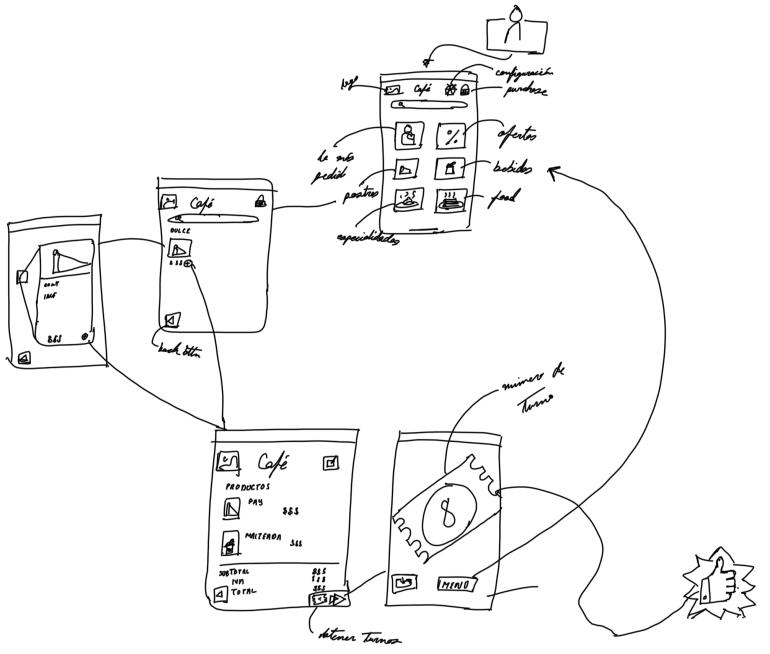
\includegraphics[width=1.00\textwidth]{C:/xampp/htdocs/Cafeteria-Menu/docImg//Img/Art/UI/UI-prototype.jpg}
	\caption{Prototipo de UI}
	\label{fig:UI-prototype}
\end{figure}

\begin{figure}[htbp]
	\centering
		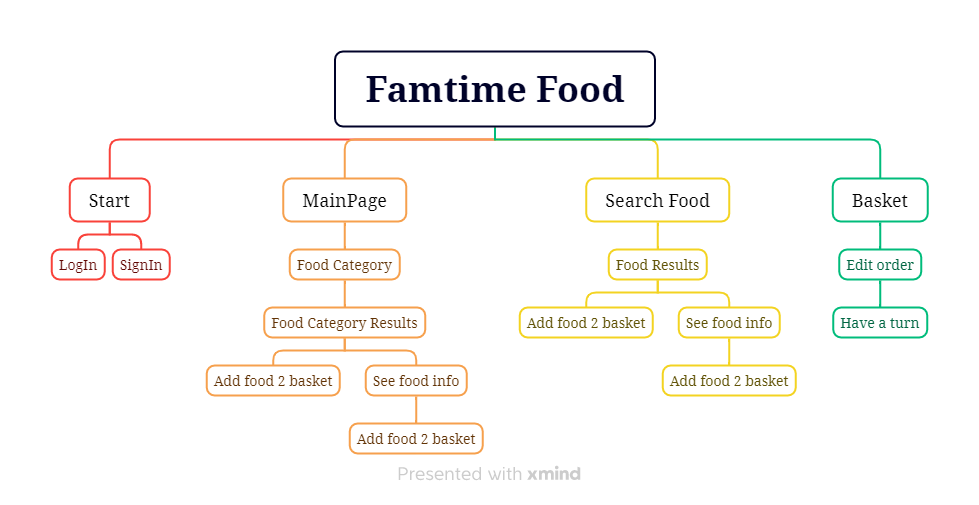
\includegraphics[width=1.00\textwidth]{C:/xampp/htdocs/Cafeteria-Menu/docImg/Img/Art/UI/UI.png}
	\caption{UI-Xmind Version}
	\label{fig:UI}
\end{figure}

\newpage
\p . . .
\newpage

\section {Manual de identidad}
\subsection {Acerca de la marca}
\p Somos una empresa con experiencia en el desarrollo de software interactivo como videojuegos y apps intercativas, ambas de toda clase de tematica, focalizando aspectos como la experiencia de usuario, creatividad, libertad, luz, oscuridad y arte.

\subsection {Nombre de la marca}
\begin{figure}[htbp]
	\centering
		
\includegraphics[width=0.90\textwidth]{C:/xampp/htdocs/Cafeteria-Menu/docImg/Img/Art/EclipseLogo.png}
	\caption{Eclipse}
	\label{fig:EclipseLogo}
\end{figure}

\subsection {Logo de la aplicacion Famtime Food}
\p El nombre de Famtime Food se refiere a la combinacion de las palabras en ingles family y food, cuyo significado es Tiempo familiar, y la palabra food es solamente par ahecr referencia y mejor enfoque al mercado objetivo.
\begin{figure}[htbp]
	\centering
		
\includegraphics[width=0.30\textwidth]{C:/xampp/htdocs/Cafeteria-Menu/docImg/Img/Art/Icon/App/Icon.png}
	\caption{App Icon}
	\label{fig:Icon}
\end{figure}


\subsection {Paletas y arte}
\begin{figure}[htbp]
	\centering
		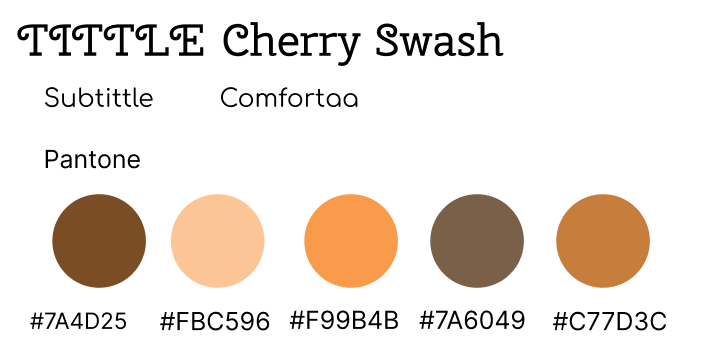
\includegraphics[width=1.00\textwidth]{C:/xampp/htdocs/Cafeteria-Menu/docImg/Img/Art/UI/Art&&Palette.png}
	\caption{Tipografia y paleta de colores de la app}
	\label{fig:Art&&Palette}
\end{figure}

\newpage

\subsection {Prototype}
\p El prototipo fue hecho mediante el uso del software de Figma

\href{https://www.figma.com/proto/jMDGvyJhrWegndvcyKfglJ/App-Cafeteria?type=design&node-id=11-2&t=SjAWG4CDYv8asbxg-0&scaling=min-zoom&page-id=0%3A1&starting-point-node-id=11%3A2&show-proto-sidebar=1}{Famtime Food Prototype}

\todo {Funcion ver info}
\p La funcion de ver mas informacion solo se encuentra representada en el producto "coca-cola light" de la seccion "Lo mas vendido" aunque esta funcion en la aplicacion se encontrara en cada uno de los productos.
	
\end{document}